
\subsection{1.25 Соединения $Ni$, $Pd$, $Pt$. Геометрия молекул в зависимости от природы лигандов, их электронное строение, способы получения и химическое поведение.}
\subsubsection*{ Соединения Ni, Pd, Pt. Геометрия молекул в зависимости от природы лигандов, их электронное строение, способы получения и химическое поведение.}

\textbf{Степени окисления}\\
$Ni$-- 0, +1, \textbf{+2}, +3 , +4\\
$Pd$-- 0, \textbf{+2}, +3, +4\\
$Pt$-- 0, \textbf{+2},\textbf{+4}, +5, +6

Сверху вниз повышается устойчивость карбонильных комплексов

\textbf{КЧ:}\\
3: $[Pt(Ph_3)_3]$\\
4:  $[Pt(Cl_4)]^{2-}$ - плоский квадрат $\Rightarrow d^8$\\
$[NiCl_4]^{2-}$ - тетраэдр $\Rightarrow d^8$

6: для $Ni[Ni(H_2O)_6]^{2+}$ и $Pd(IV), Pt(IV), [PtF_6]^{2-}$

\textbf{Получение}

Pd - отходы производства от Ni, Cu\\
Pt - саморододная в земной коре

\textbf{Химические свойства}\\
$$Pd/Pt + F_2 \rightarrow PdF_4 / PtF_6$$
$$Pd + O_2 \rightarrow PdO$$
$$Pt + HNO_3 + HCl \rightarrow H_2[PtCl_6]_6 + NO + H_2O$$
$$Pd + HNO_3 + HCl \rightarrow Pd(NO_3)_3 + NO_2 + H_2O$$

$$PtO_2\cdot 2H_2O + 2NaOh \rightarrow Na_2[Pt(OH)_6]$$
$$PtO_2\cdot 2H_2O  + HCl \rightarrow H_2[PtCl_6] + 4H2O$$
$$H_2[PdCl_6] + 2NaI \rightarrow H_2[PdCl_4] + I_2 + 2NaCl$$

\textbf{Галогениды}
$$PtCl_2 \xrightarrow{F_2, t} PtF_5$$
$$Pt \xrightarrow{F_2,t} PtF_5$$

$PdF_6$ и $PdF_5$ неизвестны, но:
$$PdF_6 + KrF_2 + O_2 \rightarrow  [O_2]^+[PdF_6]^{2-} + Kr$$

Высший галогенид $PdF_4$

$$O_2 + PtF_6 \rightarrow [O_2]^+[Pt^{+5}F_6]^-$$
$$2PtF_6 + 7CO \xrightarrow{HF, t} [Pt(CO)_4][PtF_6] + 3COF_2$$
$$PtF_6 + 6CO + SbF_5  \xrightarrow{p,t} [Pt(CO)_4][Sb_2F_{11}]_2 + 2COF_2$$

$$[Pt(CO)_4]^{2+}$$


$\textbf{Pd} : PdF_4$\\
$\textbf{Pt} : PtCl_4, PtBr_4, PtI_4$

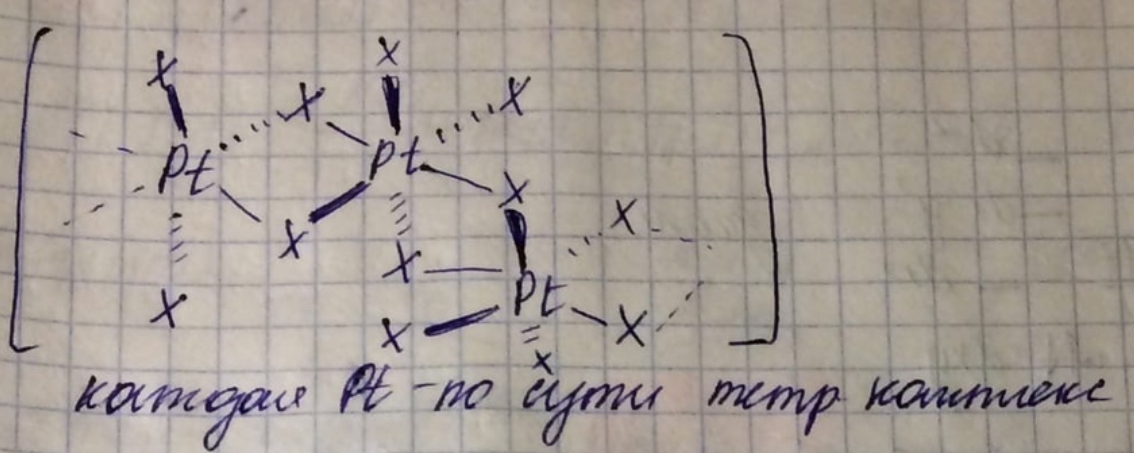
\includegraphics[scale=0.6]{25v1.png}

$$M \xrightarrow{KCl} K_2[MCl_6] (M = Pd, Pt)$$
$$K_2[PtCl_6] \xrightarrow{B_2F_3} K_2[PbF_6]$$
$$PtCl_4 \xrightarrow{HCl} H_2[PtCl_6]$$
$$PtCl_4 \xrightarrow{KCl} H_2[PtCl_6]$$
$$PtCl_4 \xrightarrow{KI} K_2[PtI_6]$$

$$trans-[PdCl_2(NH_3)_2] + Cl_2 \rightarrow trans-[PdCl_4(NH_3)_2]$$

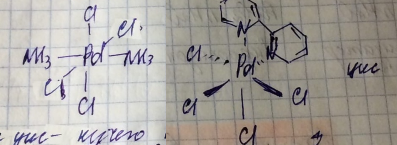
\includegraphics{25v2.png}

В цис- ничего не получится, если только N не сразу ориентированы

\textbf{Соединения Pd, Pt в с.о. +2}

$$M^{2+} + 2e \leftrightarrows M$$
$M = Ni, E^0 = -0,25 B$\\
$M = Pd, E^0 = 0,95 B$\\
$M = Pt, E^0 = 1,18 B$

$$[PtCl_6]^{2-} \xrightarrow{SO_2, HCl} H_2PtCl_4 \xrightarrow{NH_{3(konc)}} [Pt(NH_3)_4]Cl_2$$

$$[Pt(NH_3)_4]Cl_2 + [PtCl_4]^{2-} \rightarrow [Pt(NH_3)_4][PtCl_4] + 2Cl^-$$
$$[PtCl_4]^{2-} + 2NH_3\xrightarrow{aq.solution} cis-[PtCl_2(NH_3)_2] + 2Cl^-$$
$$[PtCl_4]^{2-} + 2HCl \xrightarrow{aq. solution} trans-[PtCl_2(NH_3)_2] + 2[NH_4]^+$$

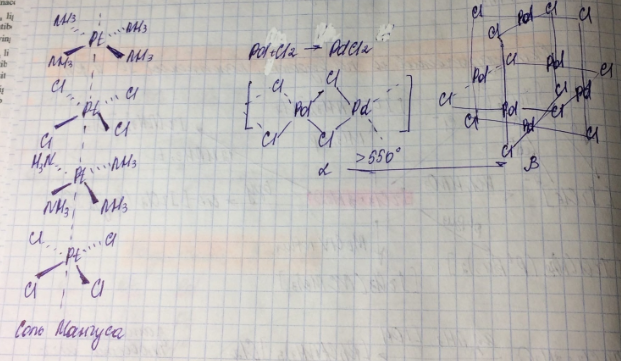
\includegraphics{25v3.png}
\\

\textbf{Транс-влияние и транс-эффект}

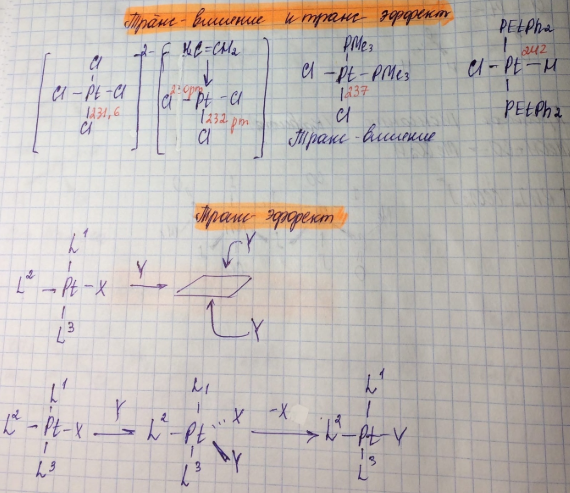
\includegraphics{25v4.png}\\
\\

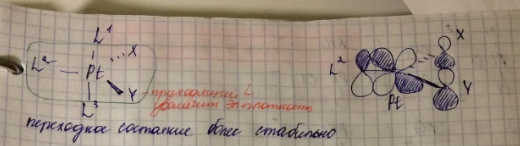
\includegraphics{25v5.png}

В основном состоянии:\\
Транс-влияние -- степень, в которой лиганды ослабляют связь в транс-положении в основном состоянии комплекса (коррелирует с $\sigma$-донорными связями, в связывании участвуют одни и те же орбитали M)

В переходном состоянии:\\
Транс-влияние коррелирует с $pi$-акцепторной способностью лиганда, "приходящий" лиганд увеличивает электронную плоскость на атоме М, акцепторный лиганд в транс-положении стабилизирует переходное состояние.

Транс-эффект можно считать комбинацией обоих эффектов

Транс $\sigma$-донор : $OH^- < NH_3 < Cl^- < Br^- < CN^- < CH_3^- <I^- < SCN^- < PR_3 , H^-$\\
Транс $\pi$-акцептор $Br^- < I^- < NCS^- < NO_2^- < CN^- < CO , C_2H_4$

$$[Pt(NH_3)_4]^{2+} + Cl^- \rightarrow [PtCl(NH_3)_2]^- \rightarrow trans-[PtCl_2(NH_3)_2]$$

$$[PtCl_4]^{2-} + NH_3 \rightarrow [PtCl_3(NH_3)]^- \rightarrow cis-[PtCl_2(NH_3)_2]$$

\textbf{Никель}

$Ni(CO)_4$ - тетраэдр, $d^{10}$\\
Цианиды: $K_2[Ni(CN)_4] \xrightarrow{Na/Hg} K_4[Ni_2(CN)_6] \xrightarrow{K/NH_{3(liq)}} K_4[Ni(CN)_4]$

С.О +2, к.ч. =4\\
$$NiBr_2 + 2KBr \rightarrow K_2[NiBr_4]$$
Устойчивый тетраэдр

Тетраэдры - только с лигандами слабого поля\\
Квадраты - с лигандами сильного поля, диамагнитны.

$$NiCl_2 + 4KCN \rightarrow 2KCl + K_2[Ni(CN)_4]$$

к.ч.=6 $[Ni(H_2O)_6]^{2+}, [Ni(NH_3)_6]^{2+}, [Ni(bipy)_3]^{2+}$\\
Антогомер $[Ni(acac)_2]$

С.О. +3\\
$d^7$ относительно устойчивы фторокомплексы, сильные окислители\\
Стабилизация $\sigma,\pi$-донорными лигандами\\
$[NiBr_3(PEt_3)_2]$ - низкоспиновый\\
$[Ni_3(CH_3COO)_6]^{3-}$

Коорд. соединение $M_3[Ni(CH-NO)_6]$

С.О.  +4

$d^5$\\
Стабилизация в гетерополисоединениях $(NH_4)_6[NiMo_9O_{32}]$\\
$[NiF_6]^{2-},  [NIO_6]$ - окислители

\textbf{Комплексы никеля}

$[NiCl_4]^{2-} [NiBr_4]^{2-}$  - тетраэдр\\
$[Ni(CN)_4]^{2-}$ - плоскоквадратный\\
$[Ni(CN)_5]^{3-}$ - тригональная бимирамида или кв.пирамида\\
$Fe(CO)_5$ - что лучше тригональная бипирамида или квадратная пирамида? Здесь - тригональная бипирамида

Зависит от природы катиона ( нарушает постулат:  признак ионных соединений -- полная независимость катиона и аниона)\\

$[NiF_6]^{4-}$ - октаэдр\\

$$NiBr_2 + PEtPh_2 \rightarrow [Br_2Ni(PEtPh_2)_2]$$

$$[Br_2Ni(PEtPh_2)_2] \leftrightarrows [Br_2Ni(PEtPh)_2]$$

$[Br_2Ni(PEtPh_2)_2]$ - зеленый, тетраэдр, парамагнитный, 2 неспаренных электрона\\

$[Br_2Ni(PEtPh)_2]$ - коричневый, плоскоквадратный, диамагнитный\\

Энергии близки их можно закристаллизовать

\textbf{Замена циклопентадиенильного кольца}

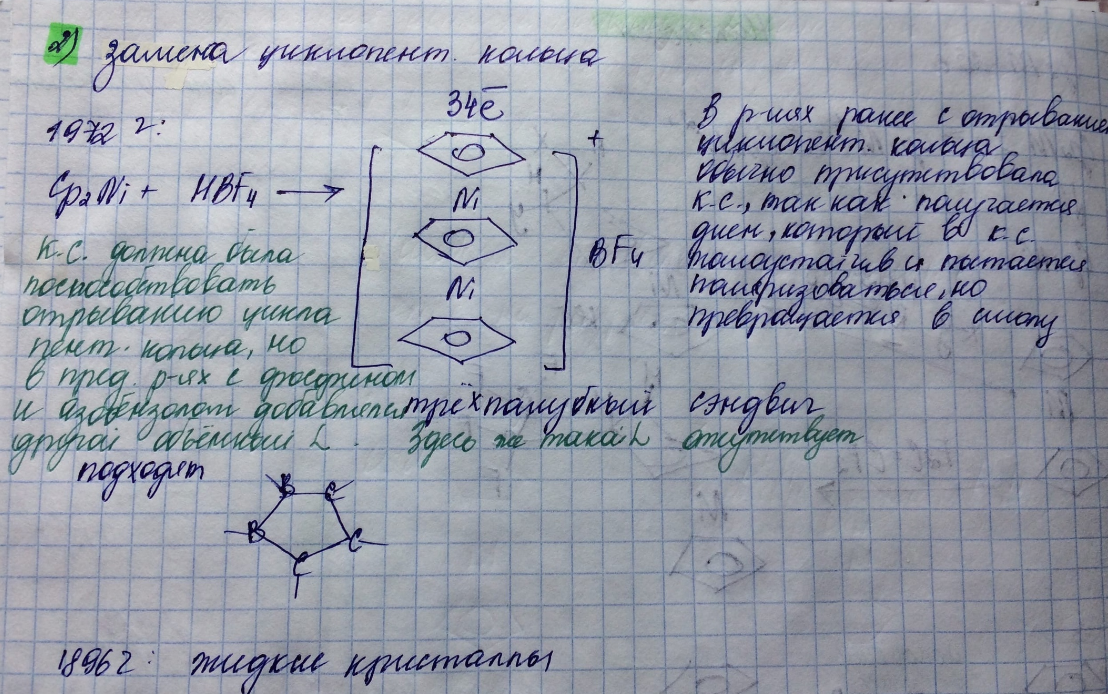
\includegraphics[scale=0.95]{25v6.png}

\textbf{Никелоцены}\\
\\

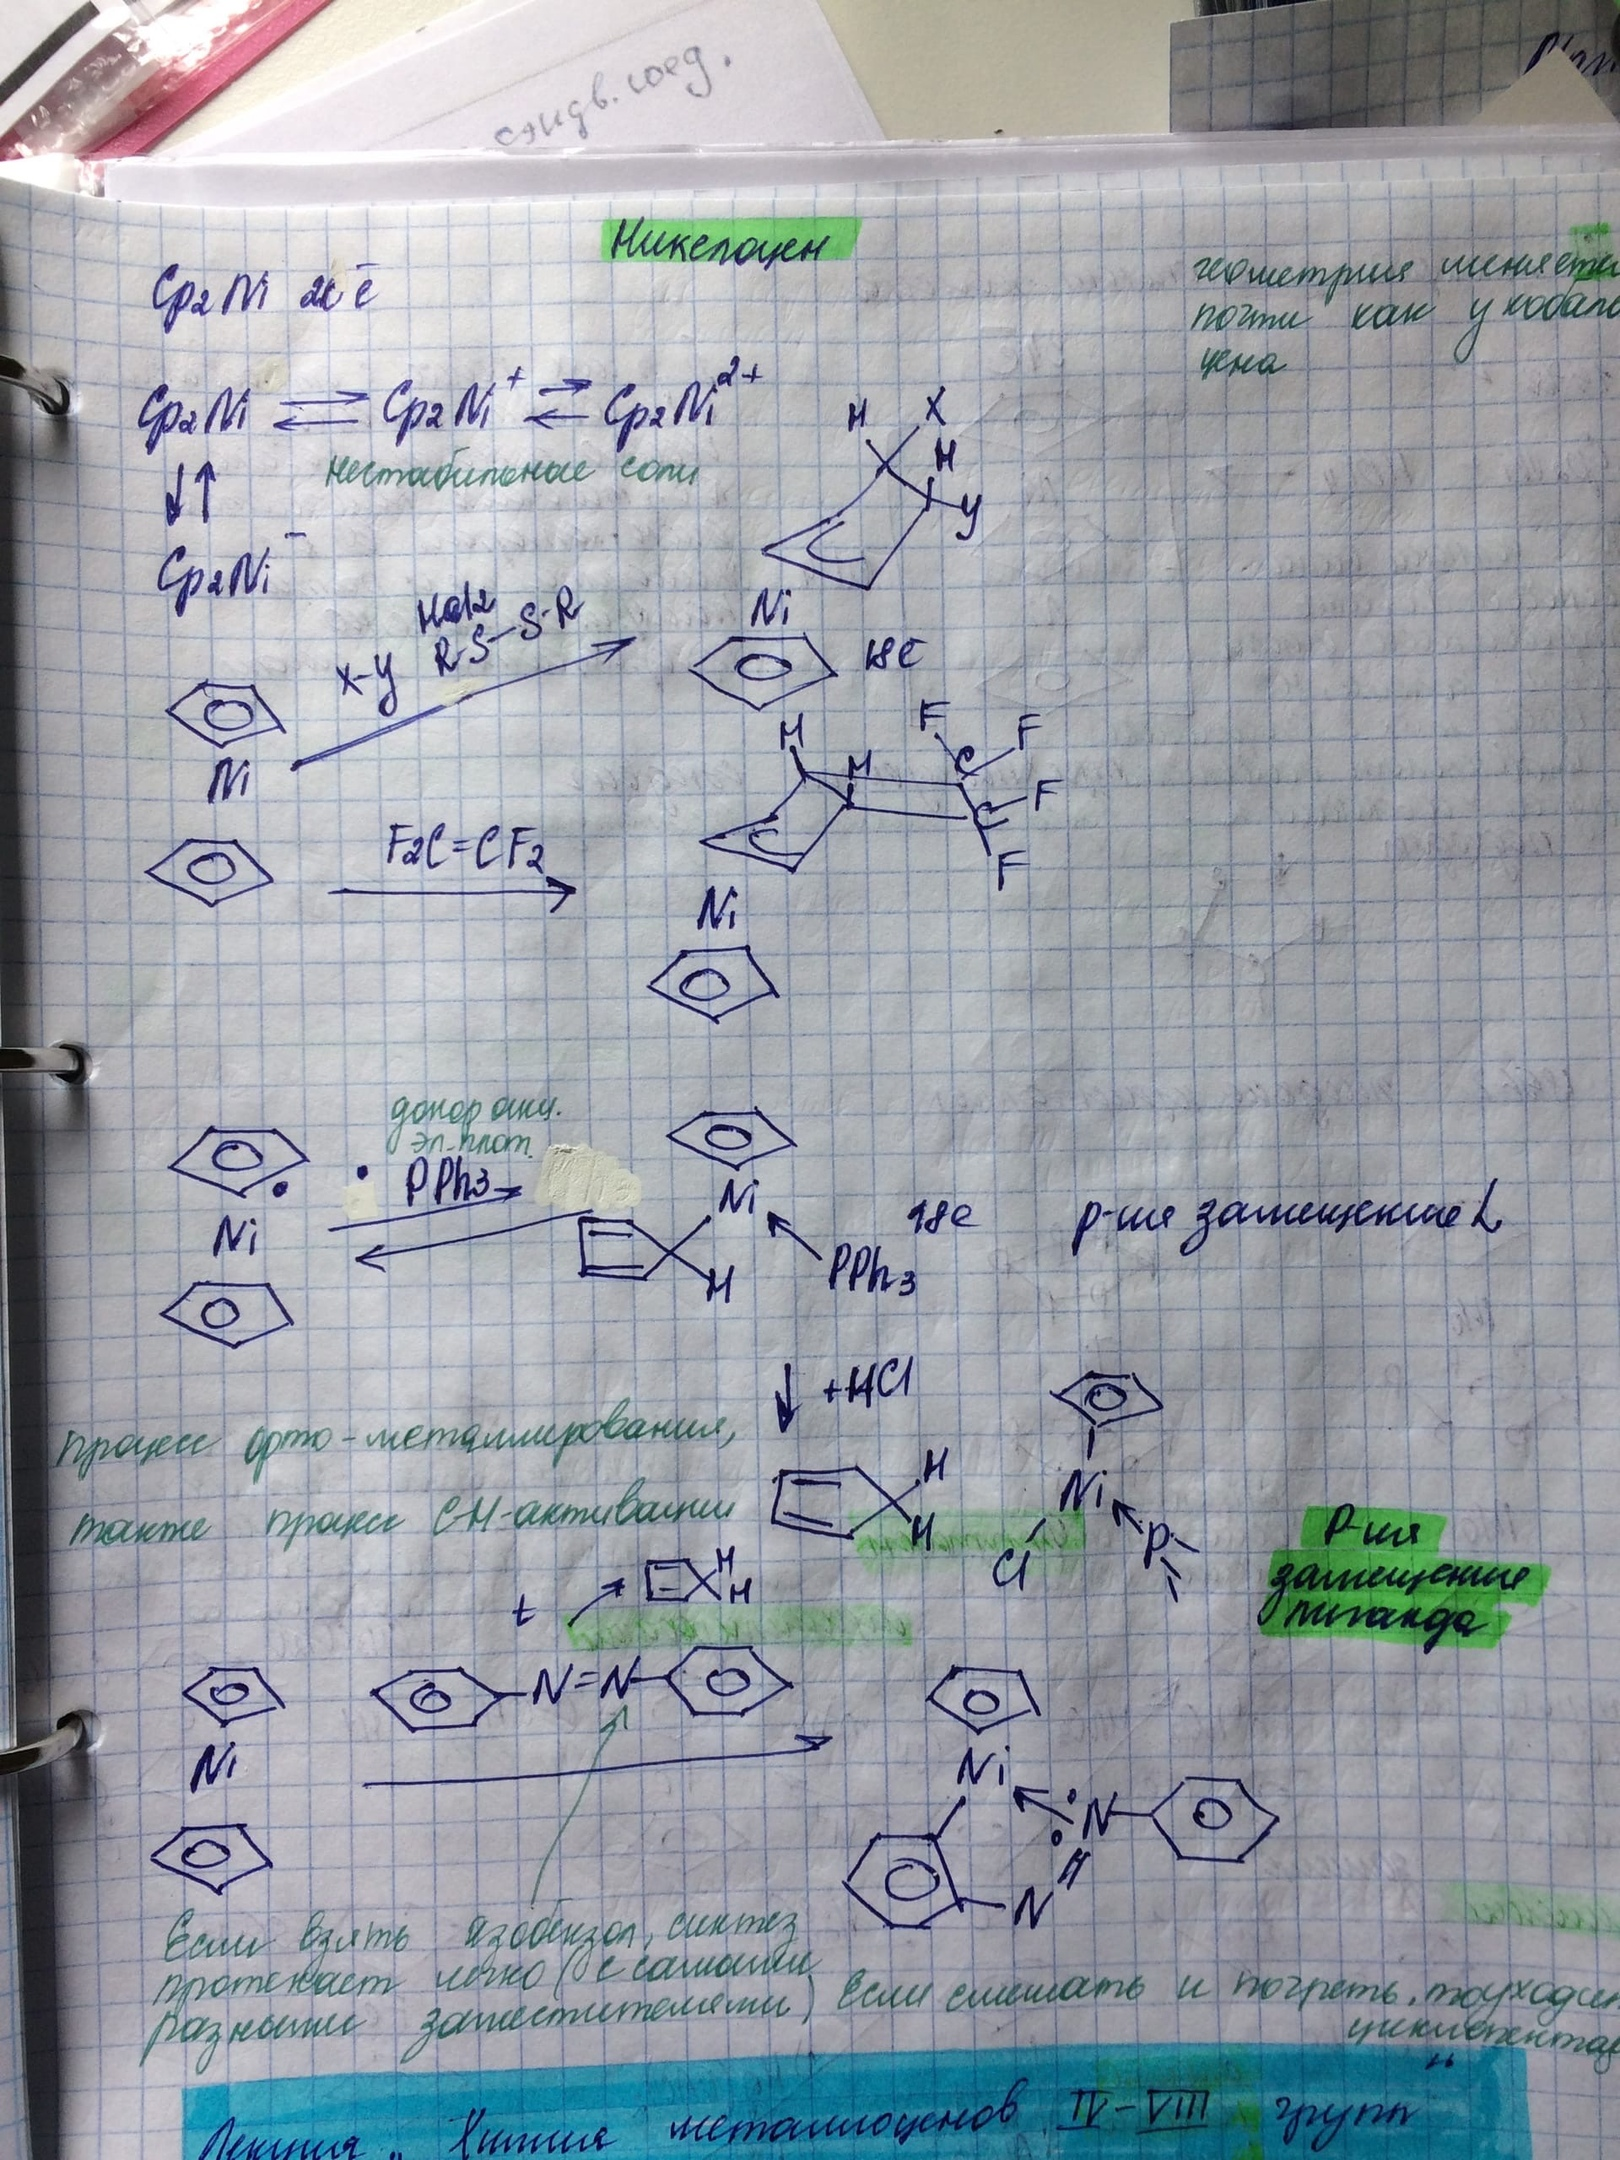
\includegraphics[scale=0.3]{25v7.png}

